\documentclass[10pt]{beamer}

\usetheme{Szeged}
\usecolortheme{rose}

\usepackage{color}
\usepackage{xcolor}
\usepackage{beamerthemeshadow}
\usepackage{mathrsfs}
\usepackage{url}
\usepackage{listings}
\usepackage{amssymb}

\definecolor{greenish}{RGB}{152,204,112}
\definecolor{redish}{RGB}{244,158,196}

\setbeamertemplate{navigation symbols}{}
\newcommand*{\LargerCdot}{\raisebox{-0.25ex}{\scalebox{3.0}{$\cdot$}}}
\expandafter\def\expandafter\insertshorttitle\expandafter{%
  \insertshorttitle\hfill%
  \insertframenumber}%\,/\,\inserttotalframenumber}


\begin{document}

\author{Kacper Sokol}
\title[Building activity recognition model]{Building activity recognition model:\\learning \texttt{Prolog} rules and extracting features from spatio-temporal data}
\institute{Department of Computer Science}
\titlegraphic{
\includegraphics[scale=.5]{../paper/gfx/UOB-logo}}
\date{\today}

\begin{frame}[plain]
\titlepage
\end{frame}

\begin{frame}[plain]
  \frametitle{Table of contents}
  \tableofcontents
\end{frame} 


\section{Background}

  \begin{frame}
    \frametitle{Healthcare issues}
    \begin{columns}
      \begin{column}{6cm}
        \begin{figure}
          \centering
          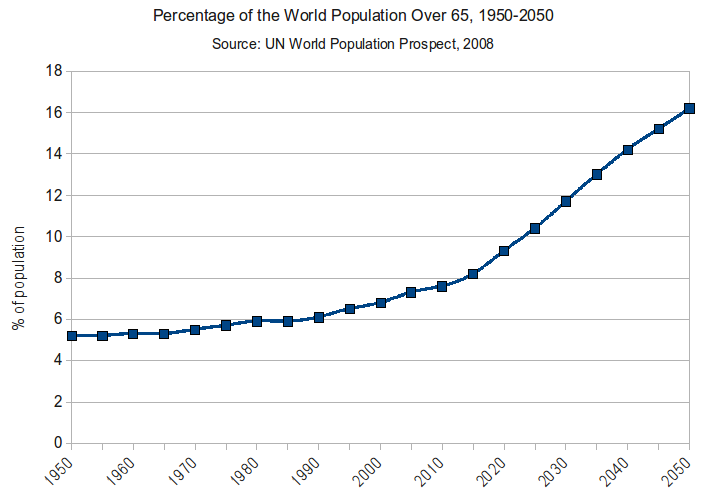
\includegraphics[width=5.5cm]{../bgSlides/gfx/populationOver65}
          \caption{Percentage of world population over 65, 1950--2050; \cite{populationAgeing}}
        \end{figure}
      \end{column}

      \begin{column}{6cm}
        \begin{block}{The Challenges}
        \begin{itemize}
          \item Global population health issues
          \item Ageing population
          \item Increasing healthcare costs
          \item Decreasing quality of life
        \end{itemize}
        \end{block}
      \end{column}

    \end{columns}

  \end{frame}

  \begin{frame}[plain]%[allowframebreaks]
    \frametitle{SPHERE project~\cite{sphere}:\\An EPSRC Interdisciplinary Research Collaboration} % (IRC)
    
      \begin{columns}

        \begin{column}{10cm}
          \begin{block}{The Technology}
            \begin{itemize}
              \item Sensors development for smart house applications
              \item \textbf{Use acquired information} to identify medical or well-being issues: predict falls, detect strokes, analyse eating behaviour, and detect periods of depression or anxiety
            \end{itemize}
          \end{block}
        \begin{block}{The Approach}
Collaboration of clinicians, engineers, designers and social care professionals as well as members of the public to develop helpful technologies:
        \begin{itemize}
          \item Focus on real-world technologies acceptable in people's homes
          \item Address real healthcare problems in a cost effective way
        \end{itemize}
      \end{block}
    \end{column}


        \begin{column}{1.5cm}
        \begin{figure}
          
\includegraphics[scale=.13]{../bgSlides/gfx/sphere} 
        \end{figure}
        \end{column}


      \end{columns}
  \end{frame}


\section{Approach}

\begin{frame}[plain]
  \frametitle{The activity recognition model}

    \begin{block}{Objectives}
    \begin{columns}
      \begin{column}{8cm}
      \begin{itemize}
        \item Learn activity recognition model
        \item Distinguish multiple occupiers
        \item Identify the most informative signal features
      \end{itemize}
      \end{column}

    \begin{column}{2cm}
      \hspace*{-1cm}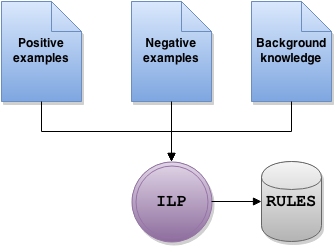
\includegraphics[width=2.5cm]{../paper/gfx/ilp}
    \end{column}

    \end{columns}
    \end{block}

    \begin{block}{Inductive Logic Programming~\cite{muggleton1994inductive,muggleton1995inverse}}
      \begin{itemize}
        \item Fusion of \emph{inductive learning} and \emph{logic programming}
        \item Induction as a basic mode of inference: build a model from available observations
        \item Powerful knowledge representation as \emph{first-order logical (parametrised) rules}---more powerful than widely used propositional logic

        \item Generate new knowledge form experience
        \item Background knowledge incorporated into model
        \item Human readable model
      \end{itemize}
    \end{block}

\end{frame}


\begin{frame}
  \frametitle{Advantages \& limitations}
  \begin{block}{Advantages}
  \begin{itemize}
    \item Background knowledge: room and sensor layout, activity structure
    \item First order logic: more complex signal features
    \item Human readable models: easy to inspect and tune
    \item Universal: one model works for variety of houses
    \item Native support for multi-class and multi-label classification
  \end{itemize}
  \end{block}

  \begin{block}{Limitations \& Challenges}
    \begin{itemize}
      \item Lack of labelled data to train and test the models
      \item Data incompleteness and noise
      \item Unbounded variables handling: time-date and real valued sensors
      \item Feature design
    \end{itemize}
  \end{block}

\end{frame}


\section{Spatio-temporal data}

\begin{frame}[fragile]
\frametitle{Smart-house data}
Smart-house data are spatio-temporal: the sensors are fixed at particular location; each sensor state change is reported with timestamp.\\[1em]

The most popular are Washington State University Center for Advanced Studies in Adaptive Systems (CASAS) datasets.
{\tiny
\begin{columns}
\begin{column}{5.4cm}
\begin{example}[\tiny CASAS smart-house output~\cite{cook2009assessing}]
\begin{figure}
\lstset{
captionpos=b,
% frame=single,
language=HTML,
breaklines=true,
% caption=CASAS dataset structure,
% label=lst:data,
float=tb,
basicstyle=\tiny
}
\begin{lstlisting}
...
2008-02-26 10:52:58.577436 M17   OFF
2008-02-26 10:52:59.792264 M17   ON
...
2008-02-26 10:53:43.512642 I02   ABSENT
2008-02-26 10:53:43.978491 I01   ABSENT
...
2008-02-26 10:53:52.112690 AD1-B 0.0421
2008-02-26 10:53:54.721822 M17   ON
...
\end{lstlisting}
\end{figure}
\end{example}
\end{column}
\begin{column}{5.4cm}
\begin{example}[\tiny Data transformation: knowledge representation]
\begin{figure}
\lstset{
captionpos=b,
% frame=single,
language=HTML,
breaklines=true,
% caption=Learnt rules,
% label=lst:rules,
float=tb,
basicstyle=\tiny
}
\begin{lstlisting}
...
sensor(m09, false, relative, 4772648).
sensor(m09, false, absolute, 120411621).
sensor(m09, false, sequence, 9).
sensor(m09, false, windowed, 0).

sensor(i08, false, relative, 5692364).
sensor(i08, false, absolute, 120411622).
sensor(i08, false, sequence, 10).
sensor(i08, false, windowed, 1).
...
\end{lstlisting}
\end{figure}
\end{example}
\end{column}
\end{columns}
}
\end{frame}

\begin{frame}[plain]
  \frametitle{Issues}

  \begin{block}{Transformation}
    \begin{itemize}
      \item Real valued sensor readings: threshold
      \item Time representation: sequence + timestamp + discretisation
      \item Ground truth: positives and negatives, generation
    \end{itemize}
  \end{block}

  \begin{block}{Data issues}
    \begin{itemize}
      \item Noise
      \item Incompleteness
      \item Lack of ground truth and precise testbed information
    \end{itemize}
  \end{block}

\vspace*{1.5em}The data issues make the model hard to learn, hence simulate the data: great control, perfect knowledge, precise ground truth, noiseless. Focus on learning and solve one problem at a time.

\end{frame}


\begin{frame}[plain]
  \frametitle{The smart-house data generator}

  \begin{block}{The generator}
      \centering\noindent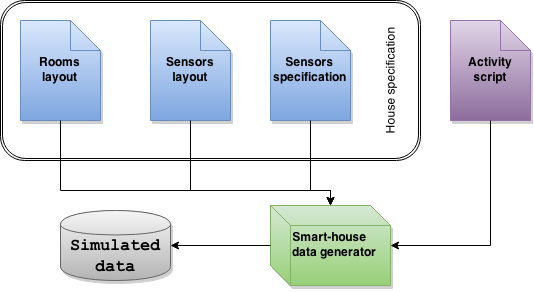
\includegraphics[width=5cm]{./gfx/gen}
  \end{block}

  \begin{block}{Advantages}
  \begin{itemize}
    \item Highly customisable: great control over the output data
    \item Precise ground truth information
    \item Works for both single and multiple residents houses
    \item Is sound
    \item Welcomed in the community for model training and testing
  \end{itemize}
  \end{block}

\end{frame}


\section{Scripted Data}

\begin{frame}
  \frametitle{Lorem}

Need to settle results evaluation\\
Compare agains the basic stats achieved with majoirty class classification\\
compare models learn on various data\\
Cross-validation\\
model-comparison\\

Basic model\\
Synthetic scripted sacas model\\
Real data\\

\end{frame} 

\begin{frame}[plain]
  \frametitle{Single resident model}
list example features\\

single resident model\\

results\\

meta rule

\end{frame} 

\section{Unscripted Data}
\begin{frame}
  \frametitle{Background}
Bathroom toilet problem\\

Synthetic data\\
Real data CASAS
\end{frame} 

\begin{frame}[plain]
  \frametitle{Two residents model}
Features\\

the model\\

results
\end{frame} 

\section{Conclusion and future work}
\begin{frame}

  \begin{block}{Conclusion}
    \begin{itemize}
      \item Good overall performance
      \item Generality
      \item Easy prediction smoothing
      \item Possibility to create complex features
      \item The power of the model lies in the features
    \end{itemize}
  \end{block}

  \begin{block}{Future work}
    \begin{itemize}
      \item Features design for more complex data
      \item Incorporate into a model ensemble
      \item Data narrative
    \end{itemize}
  \end{block}

\end{frame}

% \begin{frame}[fragile]
% \frametitle{Output}
% \begin{example}[Rules for activity recognition]
% \begin{figure}
% \lstset{
% captionpos=b,
% % frame=single,
% language=HTML,
% breaklines=true,
% % caption=Learnt rules,
% % label=lst:rules,
% float=tb
% }
% \begin{lstlisting}
% activity(Person, cooking, TimeWindow) :-
%     location(Person, TimeWindow, kitchen),
%     device(TimeWindow, hob).

% location(Person, TimeWindow, kitchen) :-
%     sensor(m08, on, absolute, TimeWindow),
%     sensor(m09, on, absolute, TimeWindow).

% device(TimeWindow, hob) :-
%     sensor(ad1-a, on, absolute, TimeWindow).
% \end{lstlisting}
% \caption{Learnt rules\label{lst:rules}}
% \end{figure}
% \end{example}
% \end{frame}  

\section*{}%References
  \begin{frame}[allowframebreaks,plain]
    \frametitle{References}
    \bibliographystyle{amsalpha}
    \bibliography{../paper/yhpargoil.bib,../bgSlides/bg.bib}
  \end{frame}

  \begin{frame}[plain]
    \centering
    \Huge Thank you!\\
    \Huge Q\&A \par
  \end{frame}

\end{document}
